%!TeX encoding = UTF-8
%!TeX program = xelatex
\documentclass[notheorems, aspectratio=54]{beamer}
% aspectratio: 1610, 149, 54, 43(default), 32

\usepackage{latexsym}
\usepackage{amsmath,amssymb}
\usepackage{mathtools}
\usepackage{color,xcolor}
\usepackage{graphicx}
\usepackage{algorithm}
\usepackage{amsthm}
\usepackage{lmodern} % 解决 font warning
\usepackage[UTF8]{ctex}


\usepackage{lipsum} % To generate test text 
\usepackage{ulem} % 下划线,波浪线

\usepackage{listings} % display code on slides; don't forget [fragile] option after \begin{frame}


\usepackage{enumerate}
\usepackage{caption}
\usepackage{subfigure}

% ----------------------------------------------
% tikx
\usepackage{framed}
\usepackage{tikz}
\usepackage{pgf}
\usetikzlibrary{calc,trees,positioning,arrows,chains,shapes.geometric,%
    decorations.pathreplacing,decorations.pathmorphing,shapes,%
    matrix,shapes.symbols}
\pgfmathsetseed{1} % To have predictable results
% Define a background layer, in which the parchment shape is drawn
\pgfdeclarelayer{background}
\pgfsetlayers{background,main}

% define styles for the normal border and the torn border
\tikzset{
  normal border/.style={orange!30!black!10, decorate, 
     decoration={random steps, segment length=2.5cm, amplitude=.7mm}},
  torn border/.style={orange!30!black!5, decorate, 
     decoration={random steps, segment length=.5cm, amplitude=1.7mm}}}

% Macro to draw the shape behind the text, when it fits completly in the
% page
\def\parchmentframe#1{
\tikz{
  \node[inner sep=2em] (A) {#1};  % Draw the text of the node
  \begin{pgfonlayer}{background}  % Draw the shape behind
  \fill[normal border] 
        (A.south east) -- (A.south west) -- 
        (A.north west) -- (A.north east) -- cycle;
  \end{pgfonlayer}}}

% Macro to draw the shape, when the text will continue in next page
\def\parchmentframetop#1{
\tikz{
  \node[inner sep=2em] (A) {#1};    % Draw the text of the node
  \begin{pgfonlayer}{background}    
  \fill[normal border]              % Draw the ``complete shape'' behind
        (A.south east) -- (A.south west) -- 
        (A.north west) -- (A.north east) -- cycle;
  \fill[torn border]                % Add the torn lower border
        ($(A.south east)-(0,.2)$) -- ($(A.south west)-(0,.2)$) -- 
        ($(A.south west)+(0,.2)$) -- ($(A.south east)+(0,.2)$) -- cycle;
  \end{pgfonlayer}}}

% Macro to draw the shape, when the text continues from previous page
\def\parchmentframebottom#1{
\tikz{
  \node[inner sep=2em] (A) {#1};   % Draw the text of the node
  \begin{pgfonlayer}{background}   
  \fill[normal border]             % Draw the ``complete shape'' behind
        (A.south east) -- (A.south west) -- 
        (A.north west) -- (A.north east) -- cycle;
  \fill[torn border]               % Add the torn upper border
        ($(A.north east)-(0,.2)$) -- ($(A.north west)-(0,.2)$) -- 
        ($(A.north west)+(0,.2)$) -- ($(A.north east)+(0,.2)$) -- cycle;
  \end{pgfonlayer}}}

% Macro to draw the shape, when both the text continues from previous page
% and it will continue in next page
\def\parchmentframemiddle#1{
\tikz{
  \node[inner sep=2em] (A) {#1};   % Draw the text of the node
  \begin{pgfonlayer}{background}   
  \fill[normal border]             % Draw the ``complete shape'' behind
        (A.south east) -- (A.south west) -- 
        (A.north west) -- (A.north east) -- cycle;
  \fill[torn border]               % Add the torn lower border
        ($(A.south east)-(0,.2)$) -- ($(A.south west)-(0,.2)$) -- 
        ($(A.south west)+(0,.2)$) -- ($(A.south east)+(0,.2)$) -- cycle;
  \fill[torn border]               % Add the torn upper border
        ($(A.north east)-(0,.2)$) -- ($(A.north west)-(0,.2)$) -- 
        ($(A.north west)+(0,.2)$) -- ($(A.north east)+(0,.2)$) -- cycle;
  \end{pgfonlayer}}}

% Define the environment which puts the frame
% In this case, the environment also accepts an argument with an optional
% title (which defaults to ``Example'', which is typeset in a box overlaid
% on the top border
\newenvironment{parchment}[1][Example]{%
  \def\FrameCommand{\parchmentframe}%
  \def\FirstFrameCommand{\parchmentframetop}%
  \def\LastFrameCommand{\parchmentframebottom}%
  \def\MidFrameCommand{\parchmentframemiddle}%
  \vskip\baselineskip
  \MakeFramed {\FrameRestore}
  \noindent\tikz\node[inner sep=1ex, draw=black!20,fill=white, 
          anchor=west, overlay] at (0em, 2em) {\sffamily#1};\par}%
{\endMakeFramed}

% ----------------------------------------------

\mode<presentation>{
    \usetheme{CambridgeUS}
    % Boadilla CambridgeUS
    % default Antibes Berlin Copenhagen
    % Madrid Montpelier Ilmenau Malmoe
    % Berkeley Singapore Warsaw
    \usecolortheme{beaver}
    % beetle, beaver, orchid, whale, dolphin
    \useoutertheme{infolines}
    % infolines miniframes shadow sidebar smoothbars smoothtree split tree
    \useinnertheme{circles}
    % circles, rectanges, rounded, inmargin
}
% 设置 block 颜色
\setbeamercolor{block title}{bg=red!30,fg=white}

\newcommand{\reditem}[1]{\setbeamercolor{item}{fg=red}\item #1}

% 缩放公式大小
\newcommand*{\Scale}[2][4]{\scalebox{#1}{\ensuremath{#2}}}

% 解决 font warning
\renewcommand\textbullet{\ensuremath{\bullet}}

% ---------------------------------------------------------------------
% flow chart
\tikzset{
    >=stealth',
    punktchain/.style={
        rectangle, 
        rounded corners, 
        % fill=black!10,
        draw=white, very thick,
        text width=6em,
        minimum height=2em, 
        text centered, 
        on chain
    },
    largepunktchain/.style={
        rectangle,
        rounded corners,
        draw=white, very thick,
        text width=10em,
        minimum height=2em,
        on chain
    },
    line/.style={draw, thick, <-},
    element/.style={
        tape,
        top color=white,
        bottom color=blue!50!black!60!,
        minimum width=6em,
        draw=blue!40!black!90, very thick,
        text width=6em, 
        minimum height=2em, 
        text centered, 
        on chain
    },
    every join/.style={->, thick,shorten >=1pt},
    decoration={brace},
    tuborg/.style={decorate},
    tubnode/.style={midway, right=2pt},
    font={\fontsize{10pt}{12}\selectfont},
}
% ---------------------------------------------------------------------

% code setting
\lstset{
    language=C++,
    basicstyle=\ttfamily\footnotesize,
    keywordstyle=\color{red},
    breaklines=true,
    xleftmargin=2em,
    numbers=left,
    numberstyle=\color[RGB]{222,155,81},
    frame=leftline,
    tabsize=4,
    breakatwhitespace=false,
    showspaces=false,               
    showstringspaces=false,
    showtabs=false,
    morekeywords={Str, Num, List},
}

% ---------------------------------------------------------------------

%% preamble
\title[muon detector simulation by using GEANT4]{muon detector simulation by using GEANT4}
% \subtitle{The subtitle}
\author{罗鑫}
\institute[SYSU]{luox46@mail2.sysu.edu.cn}

% -------------------------------------------------------------

\begin{document}

%% title frame
\begin{frame}
    \titlepage
\end{frame}

%% normal frame
\section{Introduction to geant4}
\subsection{}
\begin{frame}
  \frametitle{Introduction to geant4}
  Geant4是由欧洲核子中心(CERN)和日本高能物理中心(KEK)主导开发的蒙特卡罗辐射输运计算通用程序包,主要应用在高能物理领域,可方便模拟强相互作用、弱相互作用等高能、超高能物理过程。
\begin{block}{什么是蒙特卡罗}
  比如计算圆周率:
  \begin{itemize}
    \item 以直画圆
    \item $\pi$的理论展开公式
    \item 。。。。
  \end{itemize}
  简单的一个算法:
  \begin{itemize}
    \item 撒点
  \end{itemize}
\end{block}

\begin{block}{}
优点
\end{block}
\end{frame}
\section{Introduction to $\mu$}
\subsection{}

\begin{frame}
缪子是一种与电子相似的基本粒子,符号 $\mu^-$, 它带有 1 单位负电荷,自旋为 1/2,质量为 105 $MeV/c^2$. 缪子的反粒子是 $\mu^+$,拥有 1 单位正电荷.

地球上绝大部分自然生成的缪子都由宇宙
线中的 $\pi$ 介子产生($\pi^- \rightarrow \mu^- + \bar{\nu_u},\ \pi^+\rightarrow \mu^+ + \nu_\mu$ ).大多数缪子在海平面以上 15km 处产生.

缪子的平均寿命约为$2.2\mu s$, 准确值为 $2.1969811(22) 10^{−6} s$,缪子的衰变方式:
\begin{align}
\mu^- \rightarrow e^- + \nu_\mu + \bar\nu_\mu \\
\mu^+ \rightarrow e^+ + \bar\nu_\mu + \nu_\mu
\end{align}


\end{frame}


\section{塑料闪烁体}
\subsection{}
\begin{frame}
\frametitle{塑料闪烁体}
塑料闪烁体是有机闪烁物质在塑料中的固溶体.

当粒子进入闪烁体时,闪烁体的原子或分子受激而产生荧光。

有机闪烁体大多属于苯环结构的芳香族碳氢化合物,其发光机制主要由于分子本身从激发态回到基态的跃迁。

有机晶体主要有蒽、萘等,具有比较高的荧光效率,但体积不易做得很大。

\end{frame}


\section{PMT}
\subsection{}
\begin{frame}
\frametitle{Introduction to Photomultiplier Tubes}
光电倍增管是一种真空器件。它由光电发射阴极(光阴极)和聚焦电极、电子倍增极及电子收集极(阳极)等组成
\centering
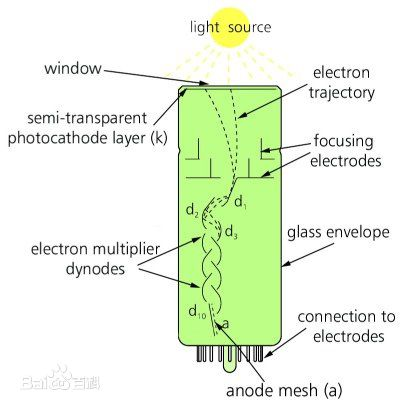
\includegraphics[scale=0.4]{../pic/pmt.jpg} 

\end{frame}

\section{符合法}
\subsection{}
\begin{frame}
符合法是研究相关事件的一种方法,相关事件是指两个或两个以上同时发生的事件,也叫符合事件。符合法要利用符合技术即用电子学的方法在不同探测器的输出脉冲中把符合事件选择出来。
\end{frame}
\section{Simulation}
\subsection{}

\begin{frame}
\center{
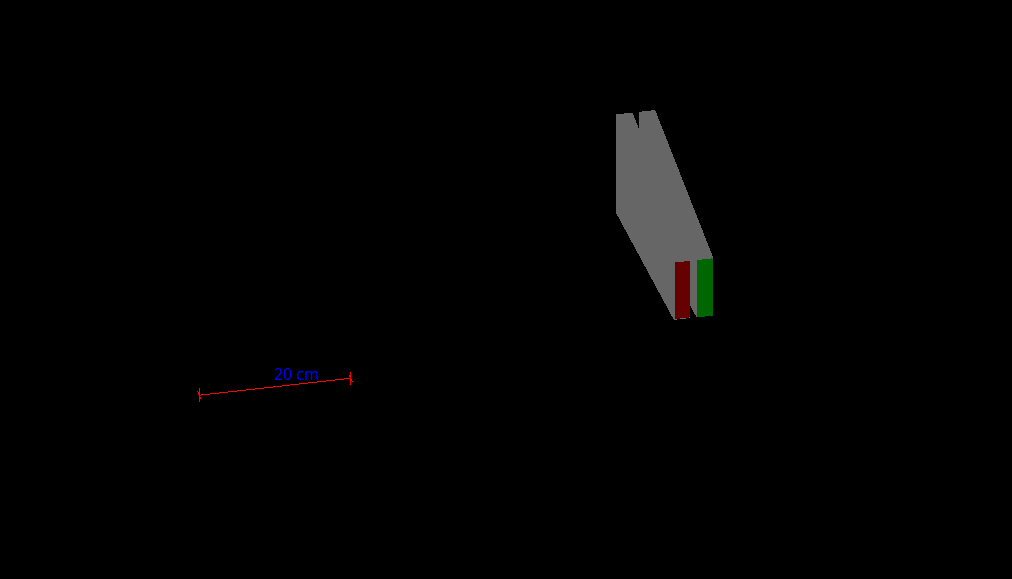
\includegraphics[height=150pt]{../pic/muondetect.png}
}
\begin{block}{Video}
\end{block}
\end{frame}

\section{result}
\subsection{detector}
\begin{frame}
\begin{figure}[htbp]
\centering
\subfigure[mu detector 沉积能量]{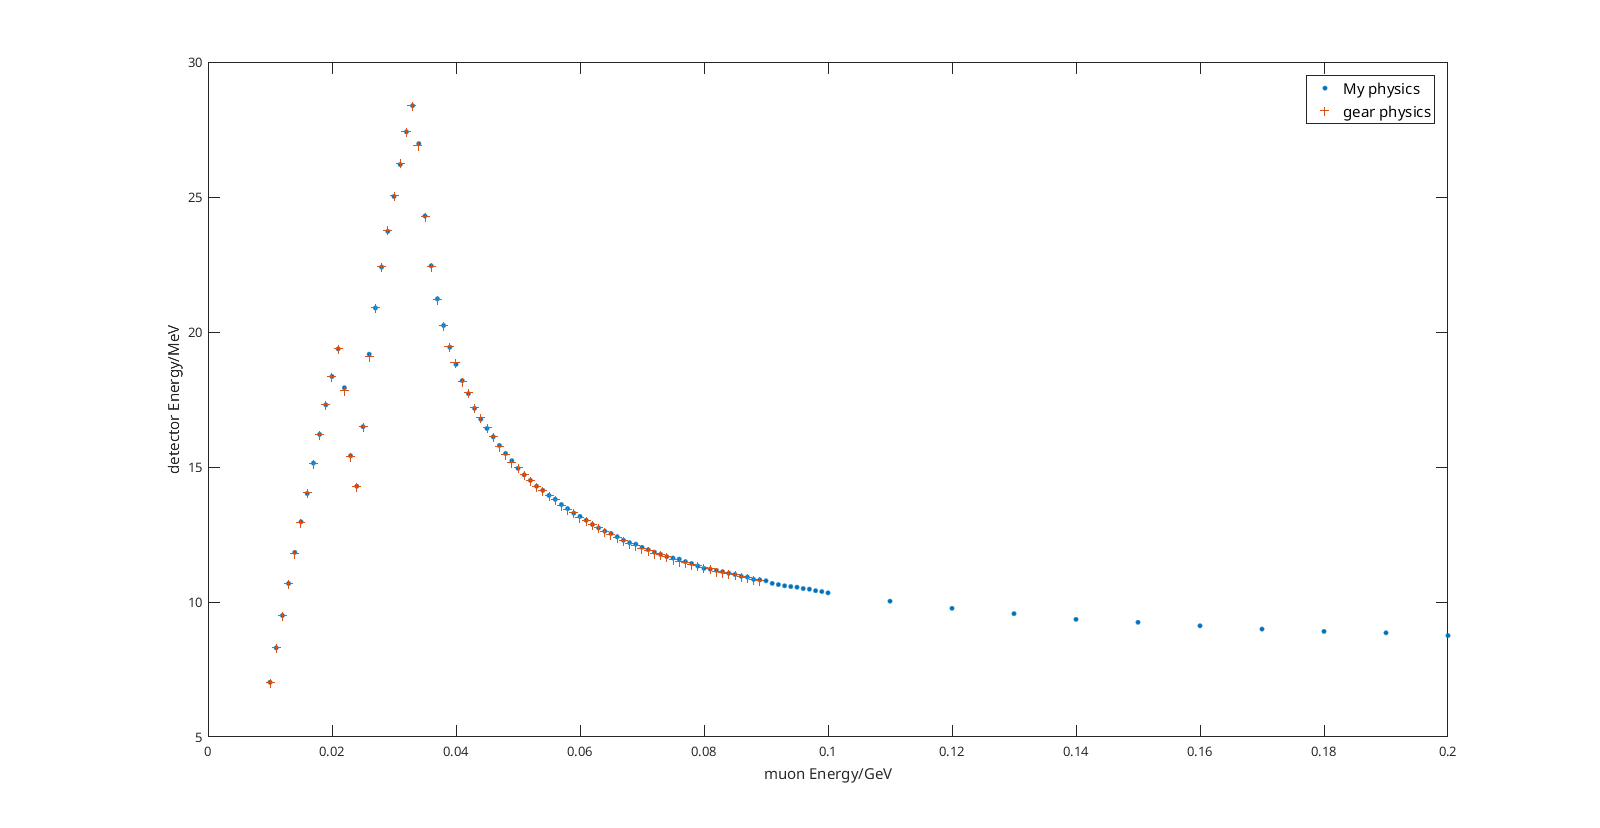
\includegraphics[scale=0.2]{../result/detector_energy.png}}
\subfigure[mu detector 穿透距离]{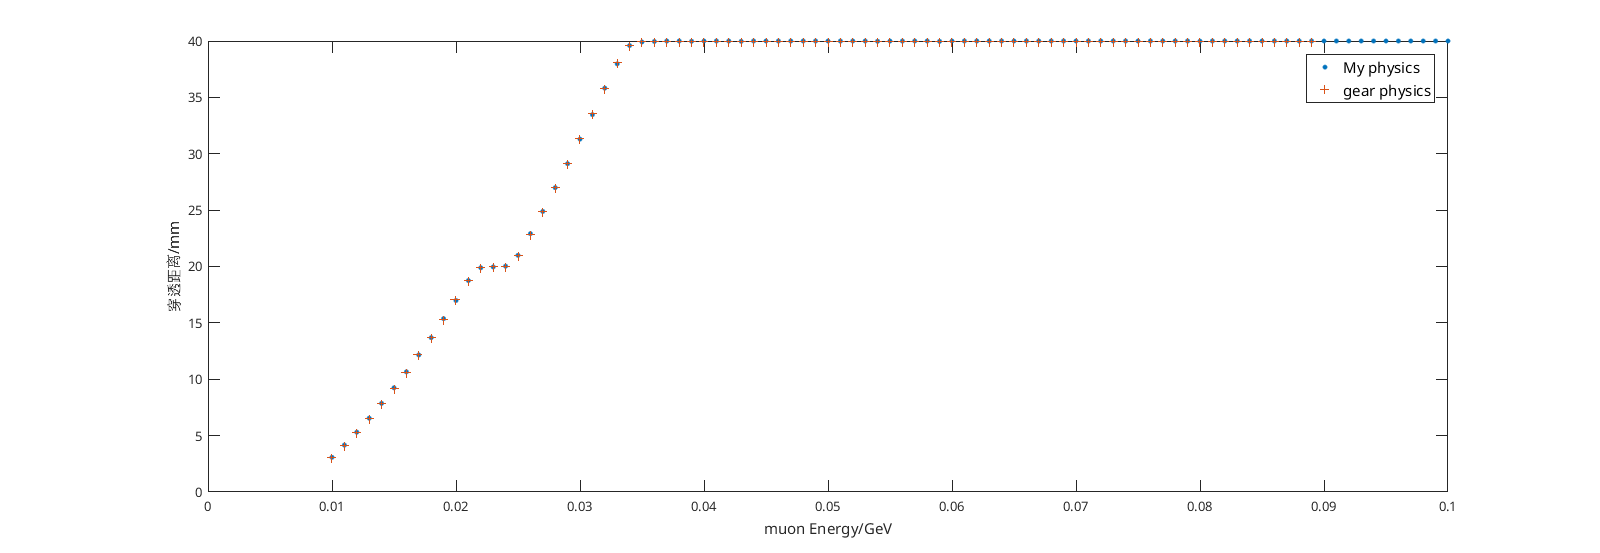
\includegraphics[scale=0.2]{../result/detector_mm.png}}
\end{figure}

\end{frame}

\section{result}
\subsection{detector}
\begin{frame}
\begin{figure}[htbp]
\centering
\subfigure[mu detector 沉积能量除以穿透距离]{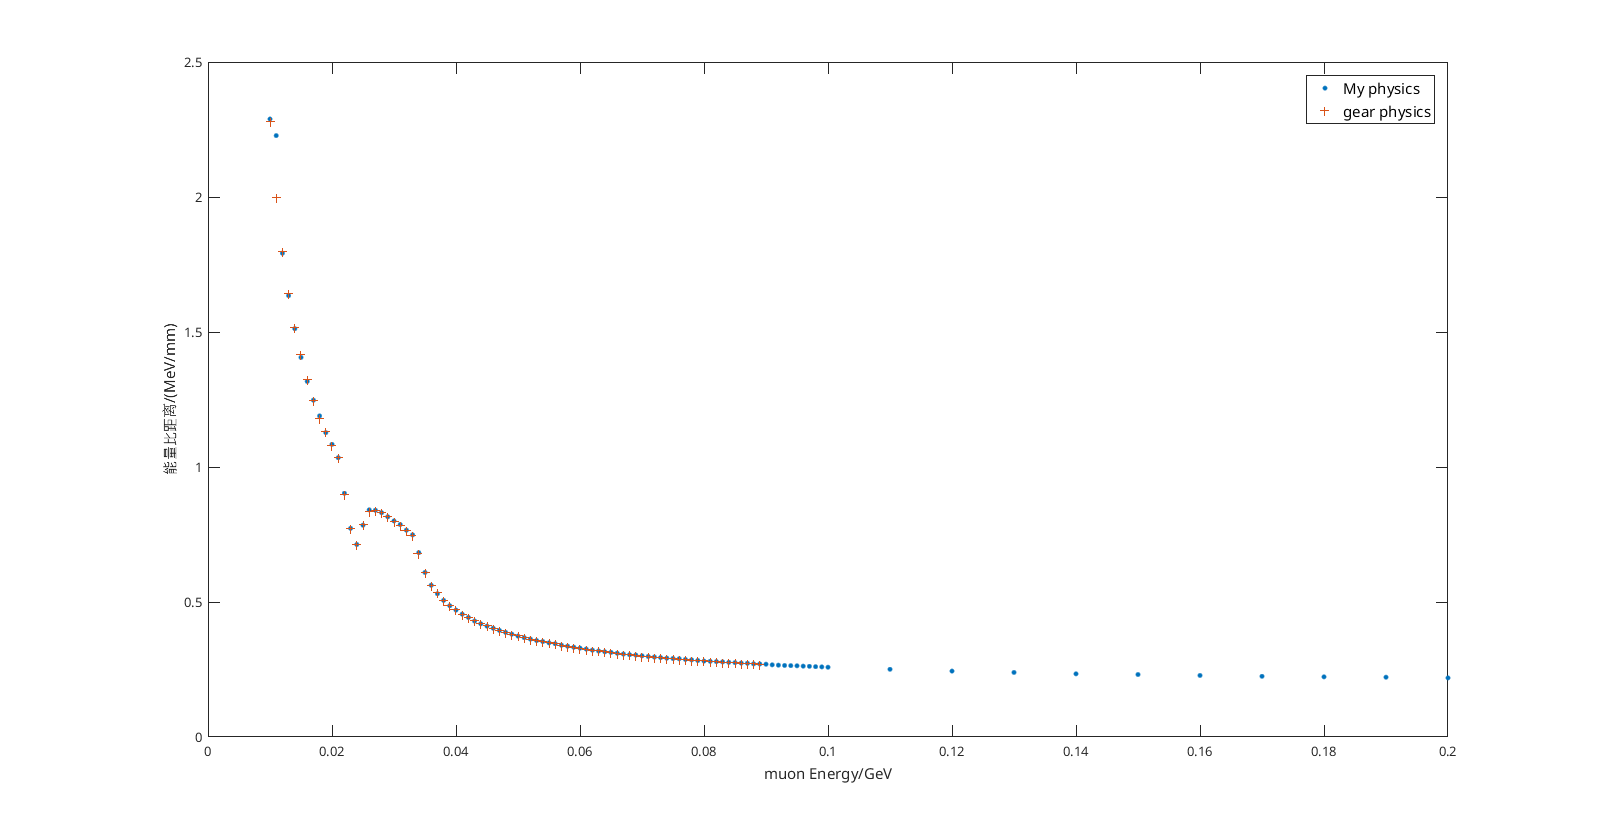
\includegraphics[scale=0.15]{../result/detector_en_mm.png}}
\subfigure[mu detector 衰变事例数]{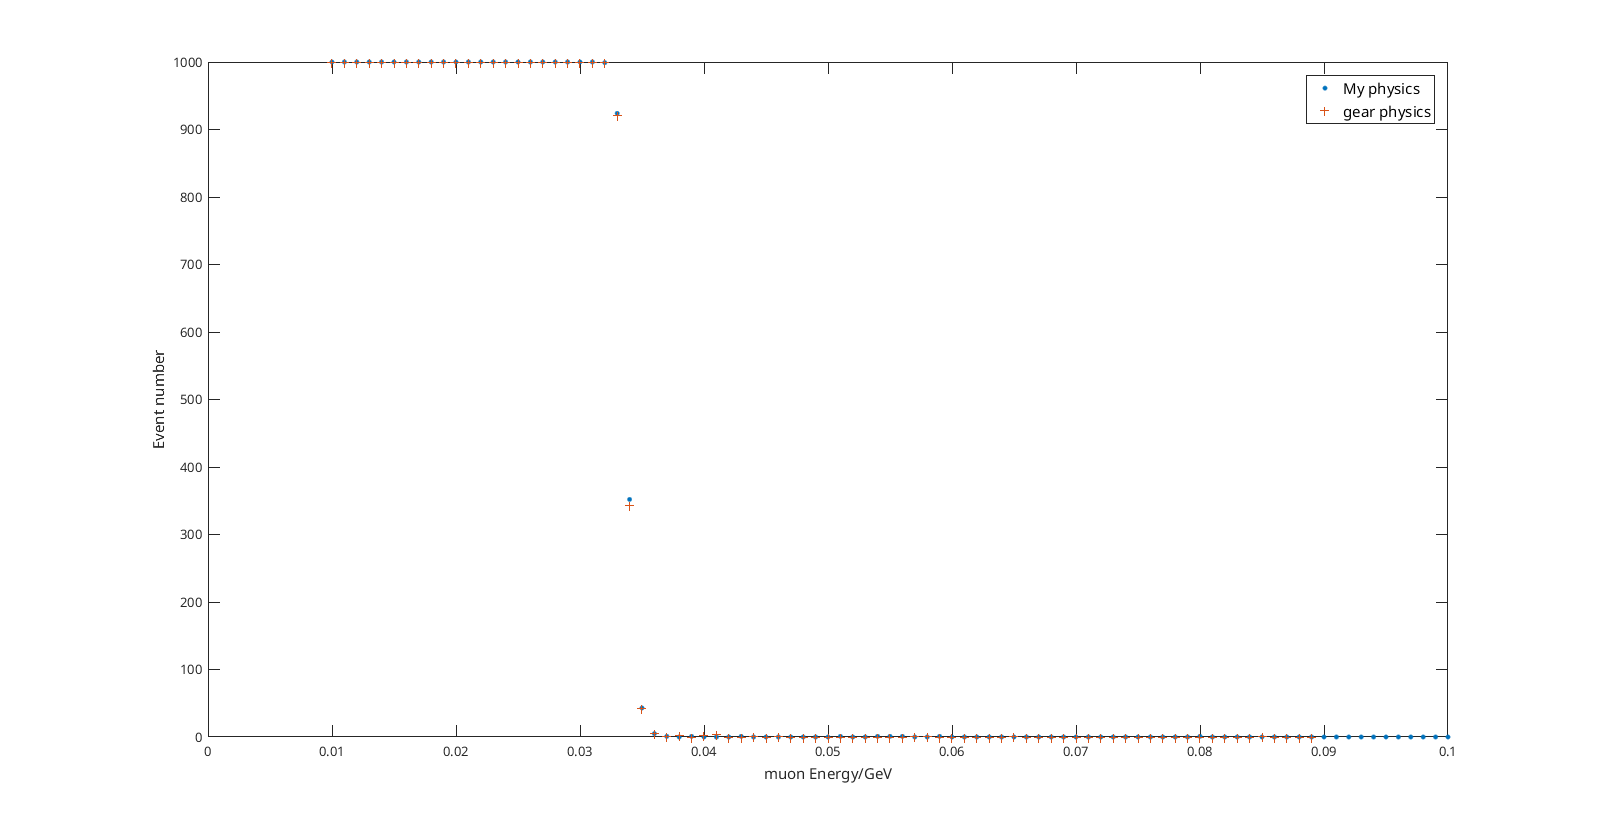
\includegraphics[scale=0.16]{../result/detector_event.png}}
\end{figure}

\end{frame}

\section{result}
\subsection{PMT}
\begin{frame}
\begin{figure}[htbp]
\centering
\subfigure[PMT 读出光子信号 与他人对比]{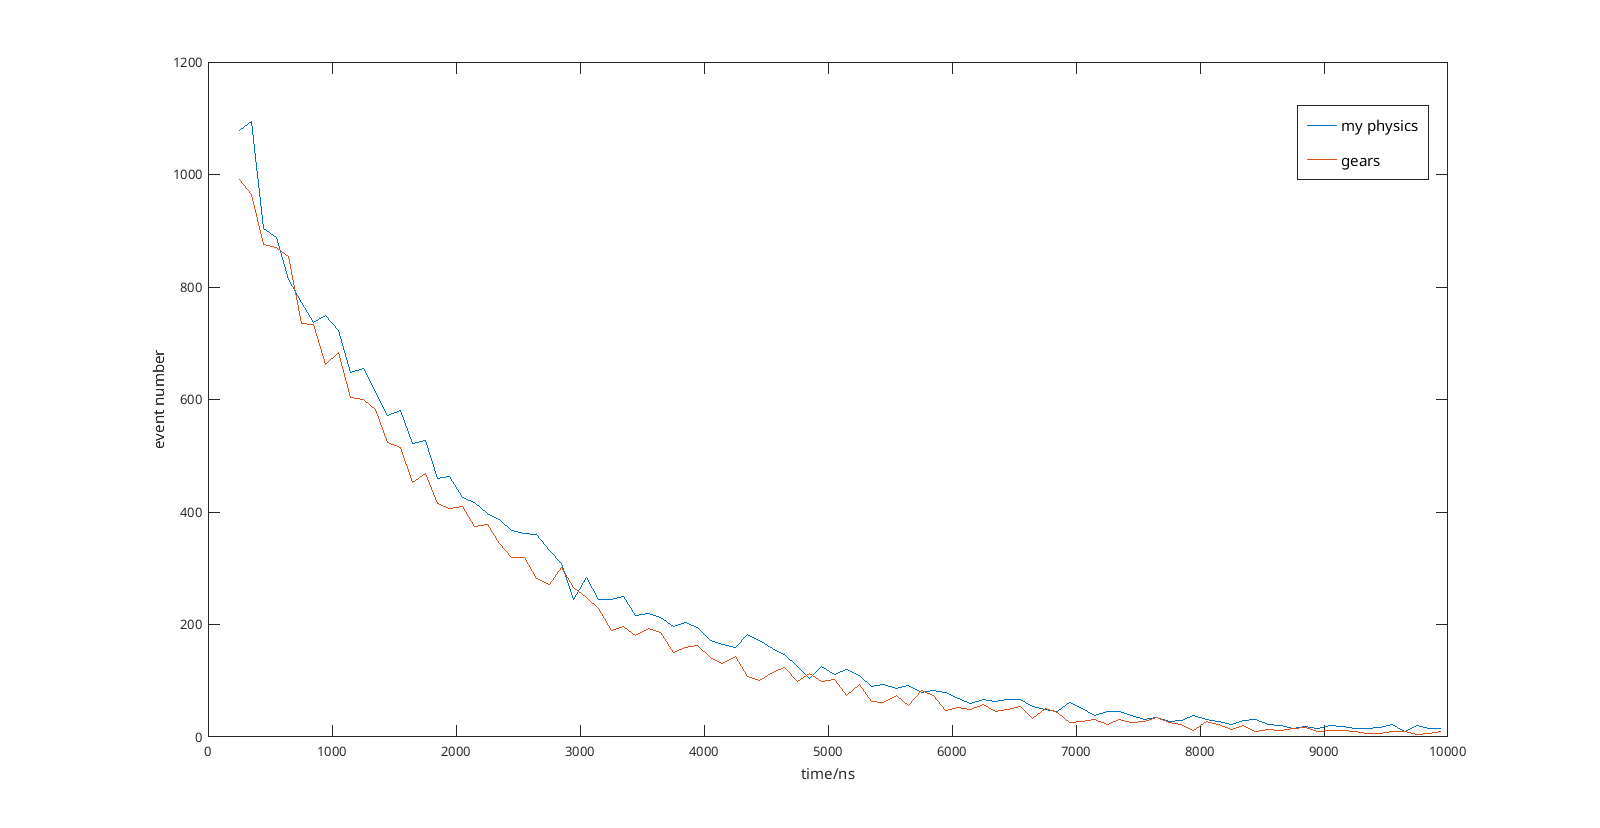
\includegraphics[scale=0.3]{../result/pmt_con.png}}
\end{figure}

\end{frame}



\section{result}
\subsection{PMT}
\begin{frame}
\begin{figure}[htbp]
\centering
\subfigure[自己的物理过程的产生 PMT 信号的拟合]{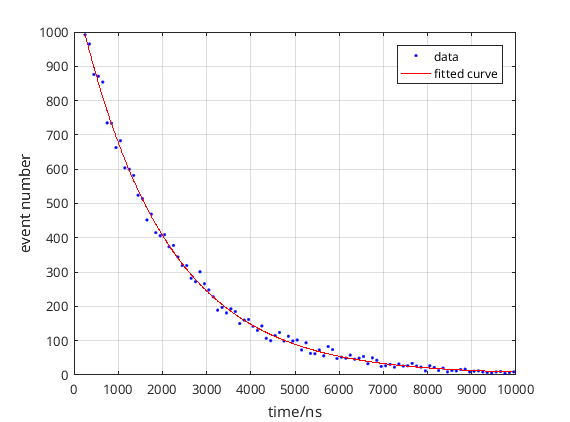
\includegraphics[scale=0.4]{../result/pmt_my.png}}
\end{figure}

$$
    f(x) = a e^{-\frac{x}{b}}+c
$$
     Coefficients (with 95\% confidence bounds):
     \begin{align}
       a =&        1126  (1112, 1140)\nonumber\\
       b =&        1959  (1913, 2006)\nonumber\\
       c =&        1.84  (-3.07, 6.75)\nonumber\\
     \end{align}

\end{frame}

\section{result}
\subsection{PMT}
\begin{frame}
\begin{figure}[htbp]
\centering
\subfigure[他人的物理过程的产生 PMT 信号的拟合]{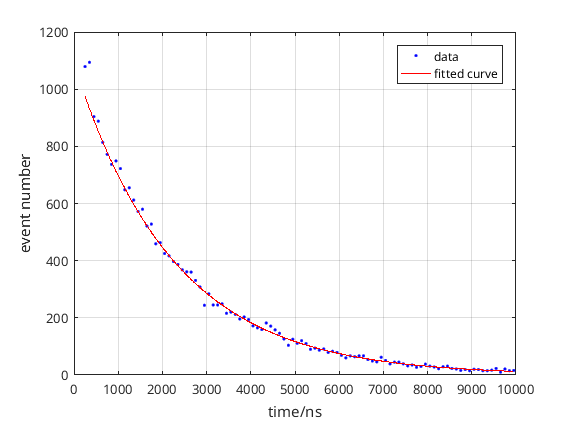
\includegraphics[scale=0.4]{../result/pmt_gear.png}}
\end{figure}

$$
    f(x) = a e^{-\frac{x}{b}}+c
$$
     Coefficients (with 95\% confidence bounds):
     \begin{align}
       a =&        1090  (1080, 1100)\nonumber\\
       b =&        2246  (2202, 2290)\nonumber\\
       c =&        -0.3383  (-4.785, 4.108)\nonumber\\
     \end{align}

\end{frame}

\section{展望}
\subsection{}
\begin{frame}
\begin{itemize}
  \item 增加光导结构
  \item 增加 PMT 复杂度,读取 PMT 产生的电子信号,模拟出实际信号
  \item 测量 $\mu$ 衰变出来的电子能谱
\end{itemize}
\end{frame}

\end{document}